\newpage\section{Sistema B + D}

Para execução dos dois sistemas em tempo real, utilizamos a biblioteca FreeRTOS disponível para Arduino.

\begin{figure}[H]
    \centering
    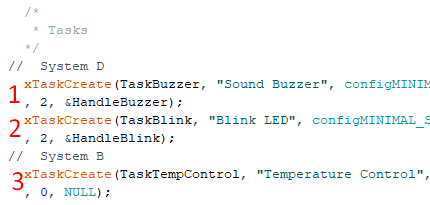
\includegraphics[scale=0.9]{images/codigo/sisBD_tasks.png}
    \caption{Criação das Tarefas}
    \label{fig:my_label}
\end{figure}

\begin{enumerate}
    \item Tarefa para Alarme Sonoro
    \begin{itemize}
        \item Prioridade -- 2
        \item Handle -- HandleBuzzer
    \end{itemize}
    \item Tarefa para Alarme Visual (LED Intermitente)
    \begin{itemize}
        \item Prioridade -- 2
        \item Handle -- HandleBlink
    \end{itemize}
    \item Tarefa para Alarme Sonoro
    \begin{itemize}
        \item Prioridade -- 0 (Iddle)
        \item Handle -- NULL (Não é necessário)
    \end{itemize}
\end{enumerate}
\newpage
Nesta junção os sistemas mantêm o mesmo funcionamento e como tal o Sistema D continua a fazer uso de Interrupts:

\begin{figure}[H]
    \centering
    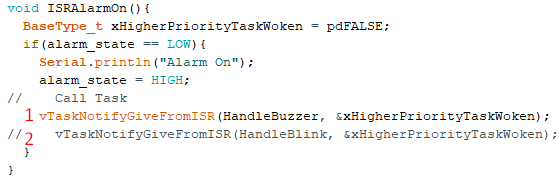
\includegraphics[scale=0.9]{images/codigo/sisBD_on.png}
    \caption{Função Interrupção (Deteção Intruso)}
    \label{fig:my_label}
\end{figure}

\begin{enumerate}
    \item Chamada/Notificação da Tarefa TaskBuzzer() (utilizando a `Handle' associada)
    \item Chamada/Notificação da Tarefa TaskBlink() (utilizando a `Handle' associada)
\end{enumerate}

\begin{figure}[H]
    \centering
    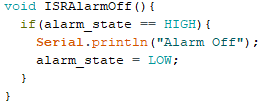
\includegraphics{images/codigo/sisBD_off.png}
    \caption{Função Interrupção (Desarme de Alarme)}
    \label{fig:my_label}
\end{figure}

Apesar da disponibilidade da biblioteca FreeRTOS, após alguma pesquisa e experiências, posso afirmar que o Arduino Uno, a placa em utilização, não está preparada a 100\% para lidar com Sistemas Operativos em Tempo Real, um dos problemas que revelou foi a não execução da TaskBuzzer() na situação da TaskBlink() estar descomentada. 
Também verifiquei que não era possível chamar qualquer uma das Tasks se a outra não fosse também criada na inicialização do programa. No entanto, foi possível executar ambas as funções mesmo que não ao mesmo tempo.

Não encontrei resposta para este problema, mesmo após uma pesquisa exaustiva.
\newpage
Assim sendo, foi feito uso da TaskBuzzer() apenas:

\begin{figure}[H]
    \centering
    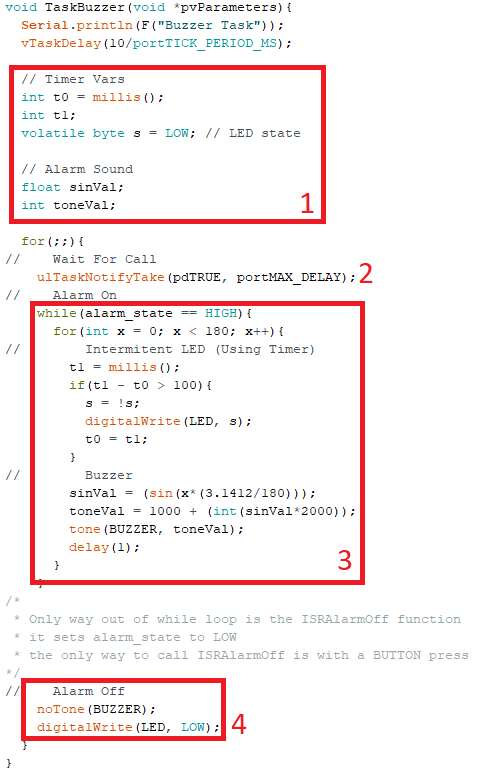
\includegraphics[scale=0.5]{images/codigo/sisBD_buzzer.png}
    \caption{Caption}
    \label{fig:my_label}
\end{figure}

\begin{enumerate}
    \item Variáveis para Alarme Sonoro e Visual
    \item A tarefa aguarda neste momento por ser chamada
    \item Execução do Alarme
    \item Execução do Desarme
\end{enumerate}